% Version  Date        Author            Notes
% 1        ?           Tobias Lutz
% 2        April 2016  Tasnad Kernetzky  Updated to new IEEEtran class (v. 1.8)
%
%
\documentclass[journal, a4paper]{IEEEtran}

% check if we are running lua(la)tex and load font related packages appropriately
\usepackage{ifluatex}
\ifluatex
    \usepackage{fontspec}
\else
    \usepackage[T1]{fontenc}
    \usepackage[utf8]{inputenc}
\fi
\usepackage{cite}
% some very useful LaTeX packages include:
%\usepackage{cite}      % Written by Donald Arseneau
                        % V1.6 and later of IEEEtran pre-defines the format
                        % of the cite.sty package \cite{} output to follow
                        % that of IEEE. Loading the cite package will
                        % result in citation numbers being automatically
                        % sorted and properly "ranged". i.e.,
                        % [1], [9], [2], [7], [5], [6]
                        % (without using cite.sty)
                        % will become:
                        % [1], [2], [5]--[7], [9] (using cite.sty)
                        % cite.sty's \cite will automatically add leading
                        % space, if needed. Use cite.sty's noadjust option
                        % (cite.sty V3.8 and later) if you want to turn this
                        % off. cite.sty is already installed on most LaTeX
                        % systems. The latest version can be obtained at:
                        % http://www.ctan.org/tex-archive/macros/latex/contrib/supported/cite/

\usepackage{graphicx}   % Written by David Carlisle and Sebastian Rahtz
                        % Required if you want graphics, photos, etc.
                        % graphicx.sty is already installed on most LaTeX
                        % systems. The latest version and documentation can
                        % be obtained at:
                        % http://www.ctan.org/tex-archive/macros/latex/required/graphics/
                        % Another good source of documentation is "Using
                        % Imported Graphics in LaTeX2e" by Keith Reckdahl
                        % which can be found as esplatex.ps and epslatex.pdf
                        % at: http://www.ctan.org/tex-archive/info/

%\usepackage{psfrag}    % Written by Craig Barratt, Michael C. Grant,
                        % and David Carlisle
                        % This package allows you to substitute LaTeX
                        % commands for text in imported EPS graphic files.
                        % In this way, LaTeX symbols can be placed into
                        % graphics that have been generated by other
                        % applications. You must use latex->dvips->ps2pdf
                        % workflow (not direct pdf output from pdflatex) if
                        % you wish to use this capability because it works
                        % via some PostScript tricks. Alternatively, the
                        % graphics could be processed as separate files via
                        % psfrag and dvips, then converted to PDF for
                        % inclusion in the main file which uses pdflatex.
                        % Docs are in "The PSfrag System" by Michael C. Grant
                        % and David Carlisle. There is also some information
                        % about using psfrag in "Using Imported Graphics in
                        % LaTeX2e" by Keith Reckdahl which documents the
                        % graphicx package (see above). The psfrag package
                        % and documentation can be obtained at:
                        % http://www.ctan.org/tex-archive/macros/latex/contrib/supported/psfrag/

%\usepackage{subfigure} % Written by Steven Douglas Cochran
                        % This package makes it easy to put subfigures
                        % in your figures. i.e., "figure 1a and 1b"
                        % Docs are in "Using Imported Graphics in LaTeX2e"
                        % by Keith Reckdahl which also documents the graphicx
                        % package (see above). subfigure.sty is already
                        % installed on most LaTeX systems. The latest version
                        % and documentation can be obtained at:
                        % http://www.ctan.org/tex-archive/macros/latex/contrib/supported/subfigure/

%\usepackage{url}       % Written by Donald Arseneau
                        % Provides better support for handling and breaking
                        % URLs. url.sty is already installed on most LaTeX
                        % systems. The latest version can be obtained at:
                        % http://www.ctan.org/tex-archive/macros/latex/contrib/other/misc/
                        % Read the url.sty source comments for usage information.

%\usepackage{stfloats}  % Written by Sigitas Tolusis
                        % Gives LaTeX2e the ability to do double column
                        % floats at the bottom of the page as well as the top.
                        % (e.g., "\begin{figure*}[!b]" is not normally
                        % possible in LaTeX2e). This is an invasive package
                        % which rewrites many portions of the LaTeX2e output
                        % routines. It may not work with other packages that
                        % modify the LaTeX2e output routine and/or with other
                        % versions of LaTeX. The latest version and
                        % documentation can be obtained at:
                        % http://www.ctan.org/tex-archive/macros/latex/contrib/supported/sttools/
                        % Documentation is contained in the stfloats.sty
                        % comments as well as in the presfull.pdf file.
                        % Do not use the stfloats baselinefloat ability as
                        % IEEE does not allow \baselineskip to stretch.
                        % Authors submitting work to the IEEE should note
                        % that IEEE rarely uses double column equations and
                        % that authors should try to avoid such use.
                        % Do not be tempted to use the cuted.sty or
                        % midfloat.sty package (by the same author) as IEEE
                        % does not format its papers in such ways.

\usepackage{amsmath}   % From the American Mathematical Society
                        % A popular package that provides many helpful commands
                        % for dealing with mathematics. Note that the AMSmath
                        % package sets \interdisplaylinepenalty to 10000 thus
                        % preventing page breaks from occurring within multiline
                        % equations. Use:
%\interdisplaylinepenalty=2500
                        % after loading amsmath to restore such page breaks
                        % as IEEEtran.cls normally does. amsmath.sty is already
                        % installed on most LaTeX systems. The latest version
                        % and documentation can be obtained at:
                        % http://www.ctan.org/tex-archive/macros/latex/required/amslatex/math/

\usepackage[belowskip=-5pt,aboveskip=5pt]{caption}
\setlength{\intextsep}{10pt plus 2pt minus 2pt}

\usepackage{algorithm,algorithmic}

% Other popular packages for formatting tables and equations include:

%\usepackage{array}
% Frank Mittelbach's and David Carlisle's array.sty which improves the
% LaTeX2e array and tabular environments to provide better appearances and
% additional user controls. array.sty is already installed on most systems.
% The latest version and documentation can be obtained at:
% http://www.ctan.org/tex-archive/macros/latex/required/tools/

% V1.6 of IEEEtran contains the IEEEeqnarray family of commands that can
% be used to generate multiline equations as well as matrices, tables, etc.

% Also of notable interest:
% Scott Pakin's eqparbox package for creating (automatically sized) equal
% width boxes. Available:
% http://www.ctan.org/tex-archive/macros/latex/contrib/supported/eqparbox/

% *** Do not adjust lengths that control margins, column widths, etc. ***
% *** Do not use packages that alter fonts (such as pslatex).         ***
% There should be no need to do such things with IEEEtran.cls V1.6 and later.


% Your document starts here!
\begin{document}

% Define document title and author
\title{Authentication based on DRAM PUFs}
\author{Chirag Mahaveer Parmar
\thanks{Advisor: Hedongliang Liu, Associate Professorship of Coding and Cryptography}}
\markboth{Seminar in Coding and Cryptography}{}
\maketitle

% Write abstract here
\begin{abstract}
One of the major security concerns regarding IoT is that of counterfeit or tampered hardware. To overcome this problem it is important to employ a hardware-intrinsic security mechanism for authentication of the device. While previous solutions like secure key storage attempt to solve this problem they only pass on the issue to the next stage. This paper outlines the use of Physically Unclonable Functions (PUFs) for hardware-intrinsic authentication. It summarizes well-known works on DRAM-based PUFs and also presents known protocols and schemes to achieve authentication on embedded devices using PUFs.
\end{abstract}

% Each section begins with a \section{title} command
\section{Introduction}
% \IEEEPARstart{}{} creates a tall first letter for this first paragraph
\IEEEPARstart{I}{n} light of the IoT era the world has seen a spike in the number of smart devices deployed in the market. These ubiquitous smart devices can be found anywhere, from toasters to cars. While they bring a lot of advantages to the table they add a profound amount of concern regarding security and privacy. \cite{EMVT12} The most prominent security concern includes counterfeit or tampered hardware. \cite{PEC06} 

Mitigating these security risks requires hardware-intrinsic security mechanisms that support authentication and identification of the device. A known solution requires cryptographic keys to be burned in at manufacturing time and then later used in symmetric/asymmetric protocols for authentication. Although this approach is susceptible to key extraction attacks giving way to cloning. Thus, Physically Unclonable Functions have been proposed as a solution to this issue.

The next section exlpains the basics of PUFs and why they are a better solution to the problem. It also dives into how DRAMs can be used as PUFs and explains various methods of doing so.

\section{Theory}
This sections goes into the basics of PUFs and workings of DRAM PUFs.
\vspace{-0.9em}
\subsection{PUFs}

In practice most PUFs are characterized by challenges and responses. A challenge is the input given to the PUF. The PUF utilizes random manufacturing variations to convert the challenge to a response. The randomness makes the response unpredictable. And because these variations cannot be controlled, even by the manufacturer, the response is unclonable on any other device. This way they attain their property of being \textbf{physically unclonable}.

\begin{figure}[!hbt]
    % Center the figure.
    \centering
    % Include the eps file, scale it such that it's width equals the column width. You can also put width=8cm for example...
    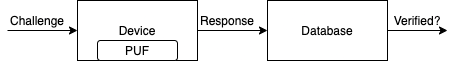
\includegraphics[scale=0.5]{figs/PUF.png}
    % Create a subtitle for the figure.
    \setlength{\belowcaptionskip}{-10pt}
    \caption{PUFS}
    % Define the label of the figure. It's good to use 'fig:title', so you know that the label belongs to a figure.
    \label{fig:tf_plot}

\end{figure}

PUFs are mainly categorized into strong PUFs and weak PUFs based on the number of unique challenge response pairs (CRPs) they can generate. Larger the CRP database, the stronger the PUF. Both kinds of PUFs have appropriate supporting authentication protocols as discussed in the next sections.

\vspace{-0.9em}

\subsection{DRAM PUFs}
There are different methods in which the process variations of DRAM can be leveraged to implement PUFs. The well-known methods are explained below.

\textbf{Startup:} In this method, the startup state of the DRAM is used for unique fingerprinting. As mentioned by Tehranipoor et al. “DRAMs have seemingly random startup values”. This is because the bitlines on DRAM are precharged to vdd/2 which makes the sense amplifier equally likely to read a ‘1’ or ‘0’. But, due to the process variations of manufacturing most bits have either a bias towards a ‘1’ or a ‘0’. Hence, the startup values of the DRAM are randomized by the random process variations. It is noted though that some bits have a neutral skew/bias i.e. they randomly switch to ‘1’ or ‘0’ over multiple startups. These bits can be used for random number generation. \cite{TEH15}

\textbf{Write Failures:} In this method, process variations affecting the write reliability are exploited. Under normal operation, the write enable signal activates the bit lines i.e. connects them to the data bus which then overrides the bit line voltage. As a result, the DRAM cells would be overwritten by the value on the data bus. For normal operation the duty cycle of the write signal is chosen such that all DRAM cells can be successfully overwritten. But for PUF operation, the duty cycle is deliberately reduced which results in some DRAM cells being overwritten while others are not. If a cell has been overwritten or not depends on the manufacturing variations. The data written under PUF operation can be treated as the challenge and a subsequent read reveals the response affected by the variations. \cite{HASH}

\textbf{Refresh Pause:} In this method, the refresh of the DRAM cells is paused to allow random decaying of the data stored in memory. \cite{SUT18} \cite{XIO16} \cite{SCH19} \cite{MISK} For normal operation DRAM cells need to be refreshed i.e. the capacitors holding the charges need to be recharged due to leakage in the circuit. If the refresh is delayed some DRAM cells decay and thereby introduce a bit flip in the stored data. Under such operation, the DRAM can be used as a PUF where the data stored before the delaying refresh can be treated as the challenge and the one after the delay as the response. An alternate method exploits data remanence properties of the DRAM, where the DRAM is completely switched off and then the cells are read. \cite{REM}

\section{Implementation Objectives}
In order to analyze the various presented methods, measurements have to be made. Almost all surveyed papers use either hamming distance and fractional hamming distance or jaccard index for measuring the properties of the PUFs. The usage of one over the other is debatable although Xiong et al claims jaccard index to be a better metric because it takes into consideration only the bits that flip as opposed to fractional hamming distance which weighs all bits of the CRP equally. 

\[ HD_{frac}(a,b) = \dfrac{HD(a,b)}{|a|} \quad\text{and}\quad J(a,b) = \dfrac{| a \bigcap b |}{| a \bigcup b |} \]

\textit{Uniqueness.} Uniqueness in PUFs is measured by comparing responses for the same challenges on different PUF instances. Greater difference in responses indicates stronger uniqueness.  The comparison is measured using either hamming distance(needs to be high) or the jaccard index(needs to be low). All surveyed work proves the uniqueness through experimentation on PUF instances of different DRAM modules, Sutar et al. goes a step further to analyze the uniqueness of different PUF instances within the same DRAM module.

% % This is how you define a table: the [!hbt] means that LaTeX is forced (by the !) to place the table exactly here (by h), or if that doesnt work because of a pagebreak or so, it tries to place the table to the bottom of the page (by b) or the top (by t).
% \begin{table}[!hbt]
%     % Center the table
%     \begin{center}
%     % Title of the table
%     \caption{Uniqueness Analysis, Refresh Pause Method}
%     \label{tab:simParameters}
%     % Table itself: here we have two columns which are centered and have lines to the left, right and in the middle: |c|c|
%     \begin{tabular}{|c|c|c|}
%         % To create a horizontal line, type \hline
%         \hline
%         % To end a column type &
%         % For a linebreak type \\

%         Avg. HD = 216 & Min. HD = 113 & Different module at t=90s \\
%         \hline
%         Avg. HD = 503 & Min. HD = 486 & Same module at t=60s \\
%         \hline

%     \end{tabular}
%     \end{center}
% \end{table}

\textit{Robustness.} Robustness of a PUF is measured by comparing the responses for the same challenges on the same PUF instances but on consequent executions. Hence robustness, in this context can also be seen as \textbf{reproducibility}. For robustness we need the HD to be close to 0 and the jaccard index to be close to 1. These measurements of robustness (same PUF instances) are further compared to the measurements of uniqueness (different PUF instances) to show \textbf{separability} or non-existence of false positives.

Robustness is also measured against temperature variations and aging. Almost all research work reports a drop in reproducibility as the temperature is increased. Although this drop is inferred differently in different conducted research. Hashemian et al which uses write failures for PUF operation claims the temperature induced variability to be not too profound thereby proving stability. Xiong et al which uses the refresh pause approach makes a relation between the temperature variation and decay rate and claims that the decay characteristics are unaffected. Xiong et al, for the above relation, suggests decreasing the refresh pause interval under increased temperature conditions. Sutar et al recommend adequate error correction and use dynamic thresholds (depending on temperature) . Aging effects on PUFs robustness is found to be negligible by most research papers.

\textit{Run-time Access.} Depending on the method used, DRAM PUFs have restricted access. For run-time access of DRAM PUFs it is important that the PUF operation doesn’t hinder the functioning of the OS and applications. The solution presented by Tehranipoor et al restricts the access to the DRAM PUF to an early boot stage because DRAM startup values cannot be accessed later. Whereas, write failures based DRAM PUFs offer the flexibility of run time access.

Refresh pause based  DRAM PUFs can offer run-time access but with modifications to the kernel in some cases. When LPDDR DRAM is being used the PUFs can be accessed at run-time due to “Partial Array Self-Refresh” functionality. \cite{SUT18} When DRAMs are split by different memory controllers they can still provide run-time access by splitting the memory per controller for OS and PUF respectively. Special case arises when the DRAM being used has none of the above features, in such case, \textit{memory ballooning} is used to reserve a DRAM region and \textit{selective memory refreshing} is used to refresh selected regions by initiating a read.\cite{XIO16}

\section{Authentication}
Most surveyed papers use the challenge response pairs for lightweight authentication of a client/prover (C) device towards a server/verifier (S) as described below.

\textit{Adversary and threat model.} It is assumed that all network traffic between client and server is observable by attackers except during the enrollment phase. This is also known as the passive attacker model and here the attacker can observe the previous PUF measurements that were passed to the server.

\begin{figure}[!hbt]
    % Center the figure.
    \begin{center}
    % Include the eps file, scale it such that it's width equals the column width. You can also put width=8cm for example...
    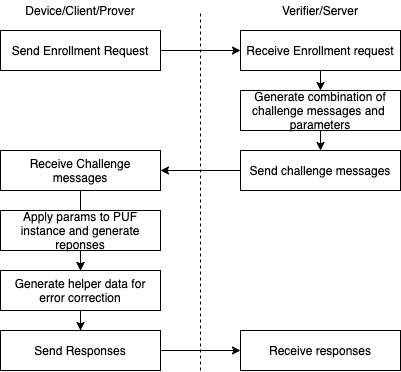
\includegraphics[scale=0.5]{figs/enrollment.png}
    \setlength{\belowcaptionskip}{-20pt}
    % Create a subtitle for the figure.
    \caption{Enrollment}
    % Define the label of the figure. It's good to use 'fig:title', so you know that the label belongs to a figure.
    \label{fig:enroll}
    \end{center}
\end{figure}

\textit{Enrollment.} The flow chart in Fig.\ref{fig:enroll} depicts the enrollment process. The enrollment phase deals with generation of the CRP database. These challenge response pairs are then either stored on a trusted secure database or distributed to verifiers in a secure manner. It has to be made sure that different verifiers receive different parts of the CRP database, otherwise one can spoof to be the device to the other.

\textit{One Way Authentication.} The flowchart in Fig.\ref{fig:one_way} depicts the one-way authentication process. In short, the server matches the device's remeasured response against the CRP database. If matches, the device is authenticated

\begin{figure}[!hbt]
    % Center the figure.
    \begin{center}
    % Include the eps file, scale it such that it's width equals the column width. You can also put width=8cm for example...
    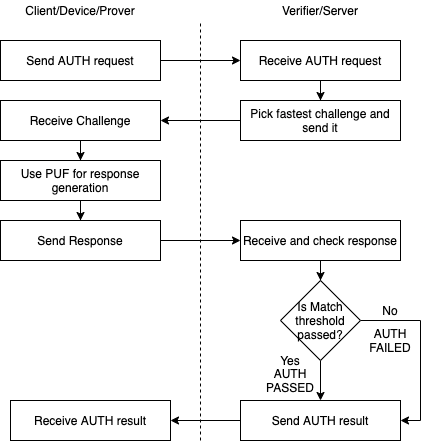
\includegraphics[scale=0.5]{figs/authentication.png}
    \setlength{\belowcaptionskip}{-20pt}
    % Create a subtitle for the figure.
    \caption{1-way Authentication}
    % Define the label of the figure. It's good to use 'fig:title', so you know that the label belongs to a figure.
    \label{fig:one_way}
    \end{center}
\end{figure}

\textit{Mutual Authentication.} This is an extension of the 1-way authentication which requires storage of CRPs in form of addresses of flipped bits rather than the bit pattern itself. The device mixes random addresses with the flipped addresses before sending the response to the server. This is done to test the knowledge of the server. The server verifies the device by counting the number of matched addresses and checking it against a threshold. The server then filters out the known flip addresses from the response and sends it to the device. The device verifies the server's response by matching it with its own response.

In both authentication protocols described above, it is important to note that:
\begin{itemize}
    \item A CRP is never used twice to prevent replay attacks. Hence a large CRP database or a strong PUF is required for continued authentication.
    \item For fast authentication it is critical to pick a CRP with the fastest possible parameters(low refresh pause interval). This requires knowledge of the PUF characteristics beforehand.
\end{itemize}

These requirements pave the way for improvements in the usage of DRAM PUFs, \textit{Parameter Reconfigurability} and \textit{Characterization}.

\textit{Parameter Reconfigurability.} The main objective of parameter reconfigurability is to increase the size of the CRP database. For this, different parameters that can change the response behaviour of the PUF have to be recognized.

Sutar et al in their work show the reconfigurability of the refresh pause interval in order to obtain new challenge-response pairs on the same PUF instance. A similar experiment is also conducted by Xiong et al and Schaller et al. After the CRPs of a particular refresh pause interval have been exhausted, the interval can be increased to a higher one depending on the number of “new” bit flips. Both these works also propose increasing the size of the PUF instance, in order to maintain the low refresh pause interval at the cost of DRAM space exhaustion. 

Apart from the refresh pause interval and the size of the PUF instance, Sutar et al and Miskelly et al demonstrate the usage of different input patterns. Sutar et al also demonstrate the effect of peripheral bits, a.k.a wrapper pattern, surrounding the block of PUF instances on the response.

With these parameters at disposal, one can reconfigure the PUF instance to generate new sets of CRP pairs and thereby increase the size of the CRP database.

\textit{Characterization:} For proper usage of the reconfiguration parameters, the challenge response behaviour must be analyzed before the authentication can take place. For achieving this the DRAM module has to be \textit{characterized}. In simple terms, characterization is the process of trying all kinds of combinations of parameters and observing the difference in responses.\cite{SUT18} After such an exhaustive experimentation the best suitable parameters are selected and the CRP database is generated accordingly. 

For example, Miskelly et al. experiment with an all ‘0’ and all ‘1’ input pattern and selects the input pattern with a higher number of bit flips. The responses for the two are biased due to the presence of true-cells and anti-cells. Apart from maximizing entropy, characterization is also used to increase robustness of the PUF. Tehranipoor et al present a solution which selects stable bits only when all neighbouring bits (spatially) are stable. Other works have also reported a 6x increase in authentication speed by optimally selecting a refresh pause interval. \cite{SUT18} \cite{SCH19}

Note that characterization is assumed to take place in a trusted and secure environment. Any information leakage of the characterization parameters reveals the characteristics of the PUF and hence make them susceptible to cloning.

\section{Secure Channel Establishment}

When a PUF cannot generate a large CRP database, it is used with a Fuzzy Extractor a.k.a Helper Data System \cite{HDS15} for secure key storage. A fuzzy extractor corrects errors in the PUF response \cite{SUT18} and enables regeneration of a cryptographic key. This way, the reproduced key can be used to setup a secure channel through symmetric protocols. Once a secure channel is established, authentication can be done through asymmetric protocols. A general construction of a fuzzy extractor contains:

\begin{itemize}
    \item \textit{Enrollment Algorithm:} The enrollment algorithm takes as input a PUF response \(X\) and a random cryptographic key \(k\) and outputs helper data \(w\).
    \item \textit{Reconstruction Algorithm:}  The reconstruction algorithm takes as input a fresh and noisy measurement of the PUF response \(X'\), and helper data \(w\), and outputs a reconstructed key \(k'\). If the noise in the PUF response is within a threshold \( k' = k\)
\end{itemize}

For using a fuzzy extractor with refresh based DRAM PUFs the decay behaviour must be discretized. Schaller et al present a viable method using refresh pause interval in which DRAM cells, during the characterization phase, are categorized into extremely fast cells \textbf{F} and slow cells \textbf{S}. The idea is that is a refresh pause interval that is greater than the decay rate of fast cells and lesser than decay rate of slow cells would guarantee a bitflip in \textbf{F} cells and no bitflip in \textbf{S} cells. In such a scenario it would be safe to mark the \textbf{F} cells as '1' an \textbf{S} cells as '0', hence, discretizing the behaviour of DRAM PUFs decay.

\begin{figure}[!hbt]
    % Center the figure.
    \begin{center}
    % Include the eps file, scale it such that it's width equals the column width. You can also put width=8cm for example...
    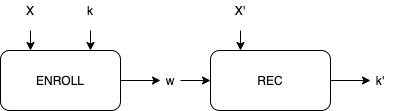
\includegraphics[scale=0.45]{figs/COM.png}
    % Create a subtitle for the figure.
    \caption{Fuzzy Extractor}
    % Define the label of the figure. It's good to use 'fig:title', so you know that the label belongs to a figure.
    \label{fig:tf_plot}
    \end{center}
\end{figure}

One of the earliest implementations of fuzzy extractors is the Code Offset Method. \cite{COM} COM uses an error correcting code at the core of its construction. The helper data \(w = X \oplus Enc(k)\), where \(Enc()\) is the encoding function of the error correcting code. The reconstructed key \(k' = Dec(X' \oplus w)\), where \(Dec()\) is the decoding function of the error correcting code. The important point to note here is that \(w\) plays the role of a syndrome. The error correcting code extracts the key \(k\) by correcting errors in \(X'\). This is clear when the formula is rewritten as \(k' = Dec(X' \oplus X \oplus Enc(k))\). Any remaining bits of the \(X' \oplus X\), if there are any, is corrected by \(Dec()\)

Using such a fuzzy extractor would also require sufficient entropy in the input \(X\). Schaller et al overcomes this problem by selecting equal number of \textbf{F} cells and \textbf{S} cells. The entropy in the input is required so that no information is leaked through the helper data, \(w\).

Another version of the COM scheme, Syndrome-COM or SCOM,\cite{COM} leverages syndrome decoding to use the input, \(X\), itself as the cryptographic key. This is done by setting the helper data to the syndrome of \(X\). During reconstruction, The expression as shown in listings below evaluates to the syndrome of the error vector which is consequently corrected by the decoder.

\begin{algorithm}
\caption{Enroll}
\begin{algorithmic}[1]
    \STATE Measure \(X \in {0,1}^{n}\)
    \STATE Compute helper data \(W = SynX\).
    \STATE Publicly store \(W\)
\end{algorithmic}
\end{algorithm}

\begin{algorithm}
    \caption{Reconstruct}
    \begin{algorithmic}[1]
        \STATE Read \(W\)
        \STATE Measure \(X' \in {0,1}^{n}\)
        \STATE \(\hat{\text{X}} = X' \oplus SynDec(W \oplus Syn(X'))\)
    \end{algorithmic}
\end{algorithm}

In this scheme the helper data \(w = Syn(X)\), where \(Syn()\) is the syndrome function. The reconstructed key \(k' = SynDec(w \oplus Syn(X'))\). 

Schaller et al in their work use the same construction of SCOM with a modification of using a key derivation function on the reconstructed input \(X'\). This is done to ensure no bias from the PUF is transferred into the cryptographic key.

Other constructions, of HDSs make use of concatenation of two linear codes. \cite{HDS15}

\[C_{1} = [n_{1}, k_{1}, d_{1}] \quad\text{and}\quad C_{2} = [n_{2}, k_{2}, d_{2}]\]

In this construction, Code \(C_{1}\) needs to maintain a high entropy, which directly translates into high cardinality or high \(k_{1}\). And, Code \(C_{2}\) needs to have a high error correction rate which directly translates to higher distance, \(d_{2}\).

\section{Conclusion}
This paper highlights why and how PUFs fulfill the demands of hardware-intrinsic authentication. It explains the well known methods of implementing PUFs on DRAMs and the advantages of DRAM PUFs. It outlines the objectives an implementation of PUF has to meet in order to be fit for use in authentication. It summarizes a simple lightweight protocol that can meet strict resource constraints for embedded processors. It also dives into the details of using PUFs for secure key storage using helper data systems (HDS) and summarizes different constructions for HDS.

% Now we need a bibliography:
\begin{thebibliography}{1}

    \bibitem{EMVT12}
    J. Viega and H. Thompson, "The State of Embedded-Device Security (Spoiler Alert: It's Bad)," in IEEE Security \& Privacy, vol. 10, no. 5, pp. 68-70, Sept.-Oct. 2012, doi: 10.1109/MSP.2012.134.

    \bibitem{PEC06}
    M. Pecht and S. Tiku, "Bogus: electronic manufacturing and consumers confront a rising tide of counterfeit electronics," in IEEE Spectrum, vol. 43, no. 5, pp. 37-46, May 2006, doi: 10.1109/MSPEC.2006.1628506.

    \bibitem{TEH15}
    Fatemeh Tehranipoor et al. 2015. DRAM based Intrinsic Physical Unclonable Functions for System Level Security. 25th edition on Great Lakes Symposium on VLSI (GLSVLSI '15). ACM, New York, NY, USA, 15–20. DOI:https://doi.org/10.1145/2742060.2742069

    \bibitem{HASH}
    M. S. Hashemian et al. "A robust authentication methodology using physically unclonable functions in DRAM arrays," 2015 Design, Automation \& Test in Europe Conference \& Exhibition (DATE), 2015, pp. 647-652, doi: 10.7873/DATE.2015.0308.

    \bibitem{SUT18}
    Soubhagya Sutar et al. D-PUF: An Intrinsically Reconfigurable DRAM PUF for Device Authentication and Random Number Generation. ACM Trans. Embed. Comput. Syst. 17, 1, Article 17 (January 2018), 31 pages. DOI:https://doi.org/10.1145/3105915

    \bibitem{XIO16}
    Xiong W. et al. (2016) Run-Time Accessible DRAM PUFs in Commodity Devices. In: Gierlichs B., Poschmann A. (eds) Cryptographic Hardware and Embedded Systems – CHES 2016. CHES 2016. Lecture Notes in Computer Science, vol 9813. Springer, Berlin, Heidelberg. https://doi.org/10.1007/978-3-662-53140-2\_21

    \bibitem{SCH19}
    A. Schaller et al., "Decay-Based DRAM PUFs in Commodity Devices," in IEEE Transactions on Dependable and Secure Computing, vol. 16, no. 3, pp. 462-475, 1 May-June 2019, doi: 10.1109/TDSC.2018.2822298.

    \bibitem{MISK}
    J. Miskelly and M. O’Neill, "Fast DRAM PUFs on Commodity Devices," in IEEE Transactions on Computer-Aided Design of Integrated Circuits and Systems, vol. 39, no. 11, pp. 3566-3576, Nov. 2020, doi: 10.1109/TCAD.2020.3012218.

    \bibitem{REM}
    Gutmann, P. Data remanence in semiconductor devices. In Proceedings of the 10th Conference on USENIX Security Symposium - Volume 10 (Berkeley, CA, USA, 2001), SSYM’01, USENIX Association.

    \bibitem{COM}
    Skoric, B., \& Vreede, de, N. (2014). The spammed code offset method. IEEE Transactions on Information Forensics and Security, 9(5), 875-884. https://doi.org/10.1109/TIFS.2014.2312851

    \bibitem{HDS15}
    J. Delvaux, D. Gu, D. Schellekens and I. Verbauwhede, "Helper Data Algorithms for PUF-Based Key Generation: Overview and Analysis," in IEEE Transactions on Computer-Aided Design of Integrated Circuits and Systems, vol. 34, no. 6, pp. 889-902, June 2015, doi: 10.1109/TCAD.2014.2370531.

\end{thebibliography}

% Your document ends here!
\end{document}
